\documentclass[
%% TIKZ_CLASSOPTION %%
tikz
]{standalone}
\usepackage{amsmath}
\usetikzlibrary{matrix}
%% EXTRA_TIKZ_PREAMBLE_CODE %%
\begin{document}
%% TIKZ_CODE %%
\usetikzlibrary{calc}
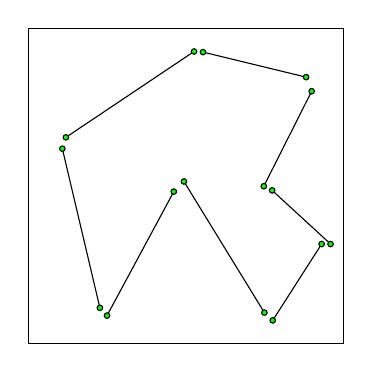
\begin{tikzpicture}[scale=4]

\coordinate (pt1)  at (0.1196,0.6535);
\coordinate (pt2)  at (0.5265,0.9261);
\coordinate (pt3)  at (0.5549,0.9242);
\coordinate (pt4)  at (0.8823,0.8447);
\coordinate (pt5)  at (0.9000,0.8000);
\coordinate (pt6)  at (0.7480,0.4984);
\coordinate (pt7)  at (0.7745,0.4851);
\coordinate (pt8)  at (0.9599,0.3148);
\coordinate (pt9)  at (0.9315,0.3148);
\coordinate (pt10) at (0.7763,0.0725);
\coordinate (pt11) at (0.7498,0.0971);
\coordinate (pt12) at (0.4943,0.5135);
\coordinate (pt13) at (0.4622,0.4813);
\coordinate (pt14) at (0.2502,0.0877);
\coordinate (pt15) at (0.2275,0.1123);
\coordinate (pt16) at (0.1083,0.6176);

\draw (0,0) rectangle (1,1);

\foreach[evaluate={\finish=int(\start+1)}] \start in {1,3,5,...,15}{
	\draw (pt\start)--(pt\finish);
}

\foreach \num in {1,2,...,16}{
	\draw[fill=green] (pt\num) circle (0.25pt);
}

% \draw[blue, very thick] (0.65145,0)--++(0,1);

% \draw[red, very thick] (0,0.56555)--++(0.65145,0);

% \draw[red, very thick] (0.65145,0.39995)--(1,0.39995);

% \draw[blue, very thick, opacity = 0.5] (0.3562,0)--(0.3562,0.56555);

% \draw[blue, very thick, opacity = 0.5] (0.32305,0.56555)--(0.32305,1);

% \draw[blue, very thick, opacity = 0.5] (0.8539,0.39995)--(0.8539,0);

% \draw[blue, very thick, opacity = 0.5] (0.8284,0.39995)--(0.8284,1);

% \coordinate (midpt1) at (0.1139,0.6356);
% \coordinate (midpt2) at (0.5407,0.9251);
% \coordinate (midpt3) at (0.8912,0.8223);
% \coordinate (midpt4) at (0.7612,0.4917);
% \coordinate (midpt5) at (0.9457,0.3148);
% \coordinate (midpt6) at (0.7631,0.0848);
% \coordinate (midpt7) at (0.4783,0.4974);
% \coordinate (midpt8) at (0.2388,0.1000);

% \draw[fill=orange, fill opacity = 0.5] 
% 	(midpt1)--
% 	(midpt2)--
% 	(midpt3)--
% 	(midpt4)--
% 	(midpt5)--
% 	(midpt6)--
% 	(midpt7)--
% 	(midpt8)--
% 	cycle;

% \foreach \num in {1,2,...,8}{
% 	\draw[fill=orange] (midpt\num) circle (0.25pt);
% }

\end{tikzpicture}
\end{document}
